\documentclass[twoside,11pt]{article}
\usepackage{jmlr2e}
\usepackage{graphicx}
\graphicspath{ {./images/} }

% Definitions of handy macros can go here

\newcommand{\dataset}{{\cal D}}
\newcommand{\fracpartial}[2]{\frac{\partial #1}{\partial  #2}}


\firstpageno{1}

\begin{document}

\title{Project 1: Machine Learning Pipeline}

\author{\name Sarah Wilson 
	   \email sawi117@jhu.edu \\
	   \phone 303-921-7225 \\
       \addr Engineering Professionals Computer Science\\
       Johns Hopkins University\\
       Baltimore, MD 21218, USA} 

\maketitle


\section{Introduction}
Regression and classification are both common tasks in the realm of Machine Learning. Regression and classification are both supervised learning problems. Supervised learning is where the system is given an input and output and then ask to learn or predict the mapping of input to out.\\ \hspace*{10mm} Regression is used to solve problems where the outcome is a number. An example of a Regression problem would be if a system needed to be built that would predict the price of a car based off of certain attributes of that car, such as, mileage, accident history and age.\\
\hspace*{10mm} Classification is used to solve problems where the outcome is a classifier or string. An example of a Classification problem would be if a system needed to built that would predict if a loan was 'high' or 'low' risk, based off of certain attributes of the person applying for that loan, such as, credit score, previous loan history and income.\\ 
\hspace*{10mm} In order to implement Regression and Classification algorithms it first must be noted that there needs to be data for these algorithms to run on. A crucial component in Machine Learning is the pre-processing of the data sets that the algorithms are intended to run on. The primary motivation behind this project was to develop a Machine Learning Pipeline that could be used to pre- process multiple unique data sets in order to pass the data to the algorithms. Due to the fact the primary objective was proper data handling the only algorithms that will be discussed in this report are: for Classification problems a Naive Majority predictor and for Regression problems the mean of an attribute in the data sets. These algorithms will be evaluated by using the \textit{k}-fold cross validation method.\\
\hspace*{10mm} The algorithms implemented for both Classification and Regression are very simple. This leads to the hypothesis that the results from these simplistic algorithms will be highly inaccurate and produce large errors.\\
\hspace*{10mm} Section 2 will discuss more examples of ways that data needs be pre-proccesed before entering the algorithms, the data-sets that were leverages, the algorithms themselves and the \textit{k}-fold cross validation method. Section 3 will present the results obtained by the Classification task using a Naive Majority predictor and for Regression task taking the mean of an attribute in the data sets. Section 4 will discuss the result that were obtain and compare that to the hypothesis that was outlined in the introduction. This report will conclude in Section 5 with a discussion of lessons learned and areas of possible future work.\\

\newpage


\section{Algorithms and Experimental Methods}
INSERT\\

\newpage
{\noindent}{\bf Data Sets}\newline
The following data sets were used during the classification and regression tasks for this project.\newline
{\bf Breast Cancer}\newline
Description: \newline
Task: Classification\newline
Predictor: Diagnosis (Malingant or Benign)\newline
Link:\newline \url{https://archive.ics.uci.edu/ml/datasets/Breast+Cancer+Wisconsin+%28Original%29}\newline
{\noindent}\textbf{Car Evaluation}\newline
Description:\newline
Task: Classification\newline
Predictor: Car Evaluation (Unacctable, Acctable, Good, Very Good)\newline
Link: \newline
\url{https://archive.ics.uci.edu/ml/datasets/Car+Evaluation}\\
{\noindent}\textbf{Congressional Vote}\newline
Description: 1984 United Stated Congressional Voting Records\newline
Task: Classification \newline
Predictor: Party (Reblican / Democrat) \newline
Link: \newline
\url{https://archive.ics.uci.edu/ml/datasets/Congressional+Voting+Records}\newline
{\noindent}\textbf{Albalone}\newline
Description: Physical merasurements of Albalone\newline
Task: Regression\newline
Predictor: Rings (int)\newline
Link: \newline
\url{https://archive.ics.uci.edu/ml/datasets/Abalone}\newline
{\noindent}\textbf{Computer Hardware}\newline
Description: Realative CPU performance data.\newline
Task: Regression\newline
Predictor: PRP\newline
Link: \newline
\url{https://archive.ics.uci.edu/ml/datasets/Computer+Hardware}\newline
{\noindent}\textbf{Forest Fires}\newline
Description: Forest Fire burn area data\newline
Task: Regression\newline
Predictor: Area (float)\newline
Link: \newline
\url{https://archive.ics.uci.edu/ml/datasets/Forest+Fires}\newline
	
\newpage

\section{Results}
The following results were obtained from the Classification task data sets.
Tables 1-3 display the results from the Breast Cancer, Car Evaluation and Congressional Vote data sets. These tables show the result from the train set and the test set during each fold of the \textit{k}-fold validation process. The tables also display the accuracy and error obtained during each fold, and the total accuracy and error as averaged across each of the 5 \textit{k}-folds. An accuracy(scale of 0-1) of 1 indicates that the train set had the most frequently occurring classifier equal to the most frequently occurring classifier in the test set. An error(scale of 0-1) of 0 indicates that the test set and train set had the same most frequently occurring classifier. Note in the Breast Cancer data set a value of 2 was mapped to the classifier of benign.\\ 

\begin{table}[h!]
	\begin{center}
		\caption{Breast Cancer: Naive Average Predictor Results}
		\label{tab:table4}
		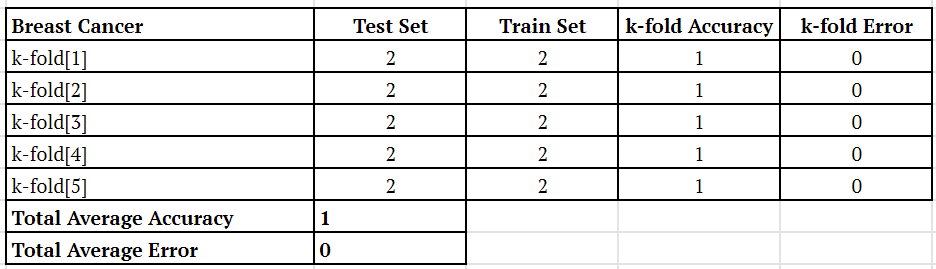
\includegraphics[scale=.6]{BC_Results}\newline
	\end{center}
\end{table}

\begin{table}[h!]
	\begin{center}
		\caption{Car Evaluation: Naive Average Predictor Results}
		\label{tab:table5}
		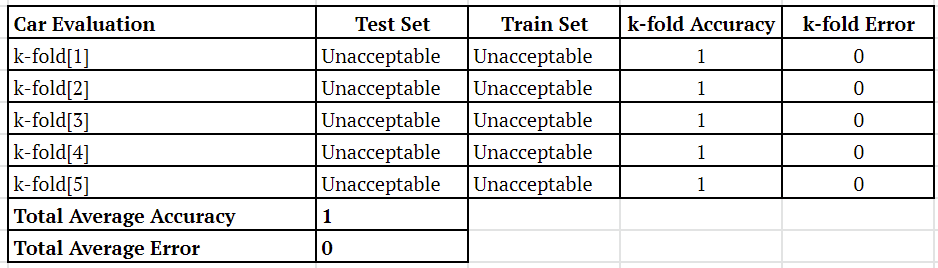
\includegraphics[scale=.6]{CE_Results}\newline
	\end{center}
\end{table}

\begin{table}[h!]
	\begin{center}
		\caption{Congressional Vote: Naive Average Predictor Results}
		\label{tab:table6}
		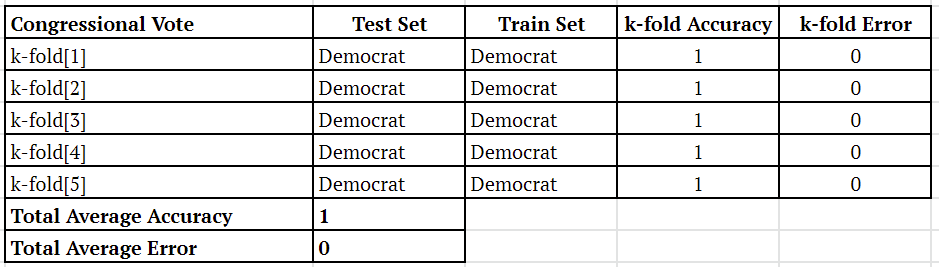
\includegraphics[scale=.6]{CV_Results}\newline
	\end{center}
\end{table}
\newpage

The following results were obtained from the Regression task data sets. Tables 4-6 display the results from the Albalone, Computer Hardware and Forest Fire data sets. These tables show the result from the train set and the test set during each fold of the \textit{k}-fold validation process.  The tables also display the error obtained during each fold, and the total error as averaged across each of the 5 \textit{k}-folds The error is the absolute error and was calculated as: $| Test Set Average - Train Set Average|$. This is meant as a measure of how far off the train set average was from the test set average. 

\begin{table}[h!]
	\begin{center}
		\caption{Breast Cancer: Naive Majority Predictor Results}
		\label{tab:table1}
		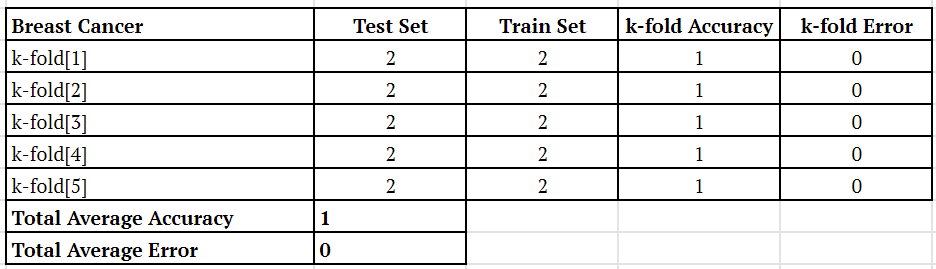
\includegraphics[scale=.6]{BC_Results}\newline
	\end{center}
\end{table}

\begin{table}[h!]
	\begin{center}
		\caption{Car Evaluation: Naive Majority Predictor Results}
		\label{tab:table2}
		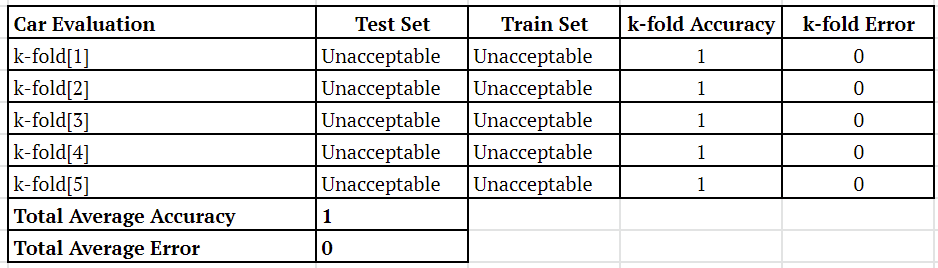
\includegraphics[scale=.6]{CE_Results}\newline
	\end{center}
\end{table}

\begin{table}[h!]
	\begin{center}
		\caption{Congressional Vote: Naive Majority Predictor Results}
		\label{tab:table3}
		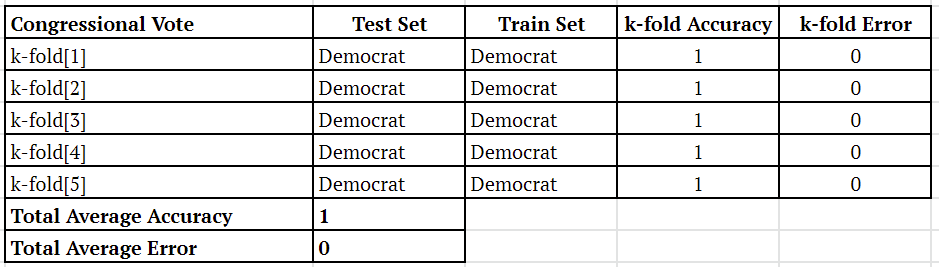
\includegraphics[scale=.6]{CV_Results}\newline
	\end{center}
\end{table}



\newpage

\section{Discussion}
The hypothesis was that since the algorithms implemented for Classification and Regression were very simplistic the prediction results from these algorithms will be highly inaccurate and produce large errors.

\newpage

\section{Conclusion}

\newpage



\vskip 0.2in
\bibliography{sample}

\end{document}